\documentclass{scrartcl}

\usepackage[linear]{handout}
\usepackage{bbm}
\usepackage{circuitikz}
% \usepackage{mlmodern}
% \usepackage{gfsartemisia}
\ihead{\sffamily\bfseries\footnotesize{Experiment 03}}
\ohead{\sffamily\footnotesize\textbf{}} 

\title{
        \Large\textsc{PH3204: Electronics Lab} \\
        \vspace{10pt}
        % \Large\textsc{Experiment 02} \\
        % \vspace{0.1cm}
        \Huge \textbf{Study of Operational Amplifier(OPAMP)} \\
}

% \subtitle{}

\author{Sabarno Saha \\ \texttt{22MS037} \\ Grp. B-10}

\date{\normalsize
        \textit{Indian Institute of Science Education and Research, Kolkata, \\
        Mohanpur, West Bengal, 741246, India.}
        % \vspace{10pt}
        % \today
}
\newcommand{\1}{\mathbbm{1}}
\newcommand{\ichi}{\tilde{\chi}}
\newcommand{\irho}{\tilde{\rho}}
\newcommand{\ihsr}{\tilde{H}_{SR}}
\newcommand{\G}{\Gamma}
\newcommand{\iG}{\tilde{\Gamma}}
\newcommand{\is}{\tilde{s}}
\newcommand{\h}{\mathbb{H}}
\newcommand{\nbar}{\bar{n}}

\graphicspath{{./code/}}

\begin{document}
\maketitle
\tableofcontents
\newpage
\section{Aim}
In this experiment, we will study the working of an operational amplifier (OPAMP) and its applications in various circuits, namely
its use as an inverting amplifier, a non-inverting amplifier, an adder and a subtractor.
\section{Theory}
Operational Amplifier are electronic components used to amplify signals. 
\begin{figure}[h]
    \centering
    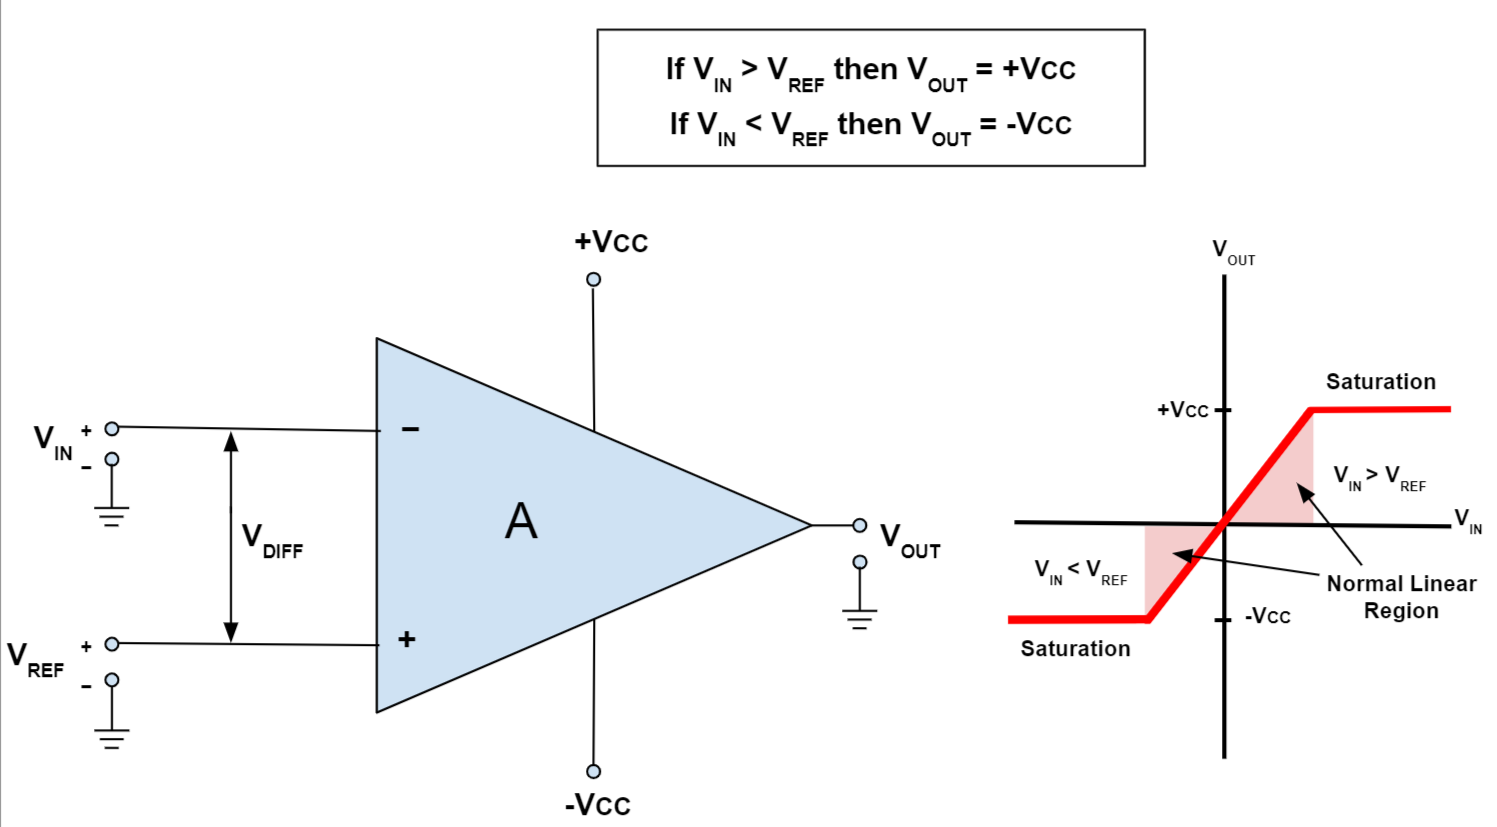
\includegraphics[width=0.74\textwidth]{opamp.png}
    \caption{OP-AMP with characterisitic curve, Source :The Internet}
\end{figure}
OP-AMPS run on the principle of virtual ground and have a very high gain. The gain of an op-amp is very high and is given by
\begin{align*}
    A = \frac{V_o}{V_i} = \infty
\end{align*}

where $V_o$ is the output voltage and $V_i$ is the input voltage. The op-amp has two inputs, the inverting input and the non-inverting input. 
The inverting input is denoted by $V^-$ and the non-inverting input is denoted by $V^+$. 
 The output voltage of the op-amp is given by
\begin{align*}
    V_o = A(V^+ - V^-)
\end{align*}
where $A$ is the open loop voltage gain of the op-amp.
The OP-AMP draws voltage from the power supply often called $V_cc$ or the source voltage. The $V_i$ vs $V_o$ 
characteristic of an op-amp is shown in the figure above. The op-amp has a linear region where the output voltage is linearly proportional to the input voltage.
In practice, op-amps have a large gain therefore this linear region has slope almost infinite.
The op-amp then switches to the saturation voltage which is the voltage supplied by the power supply.

\par
\begin{figure}[H]
    \centering
    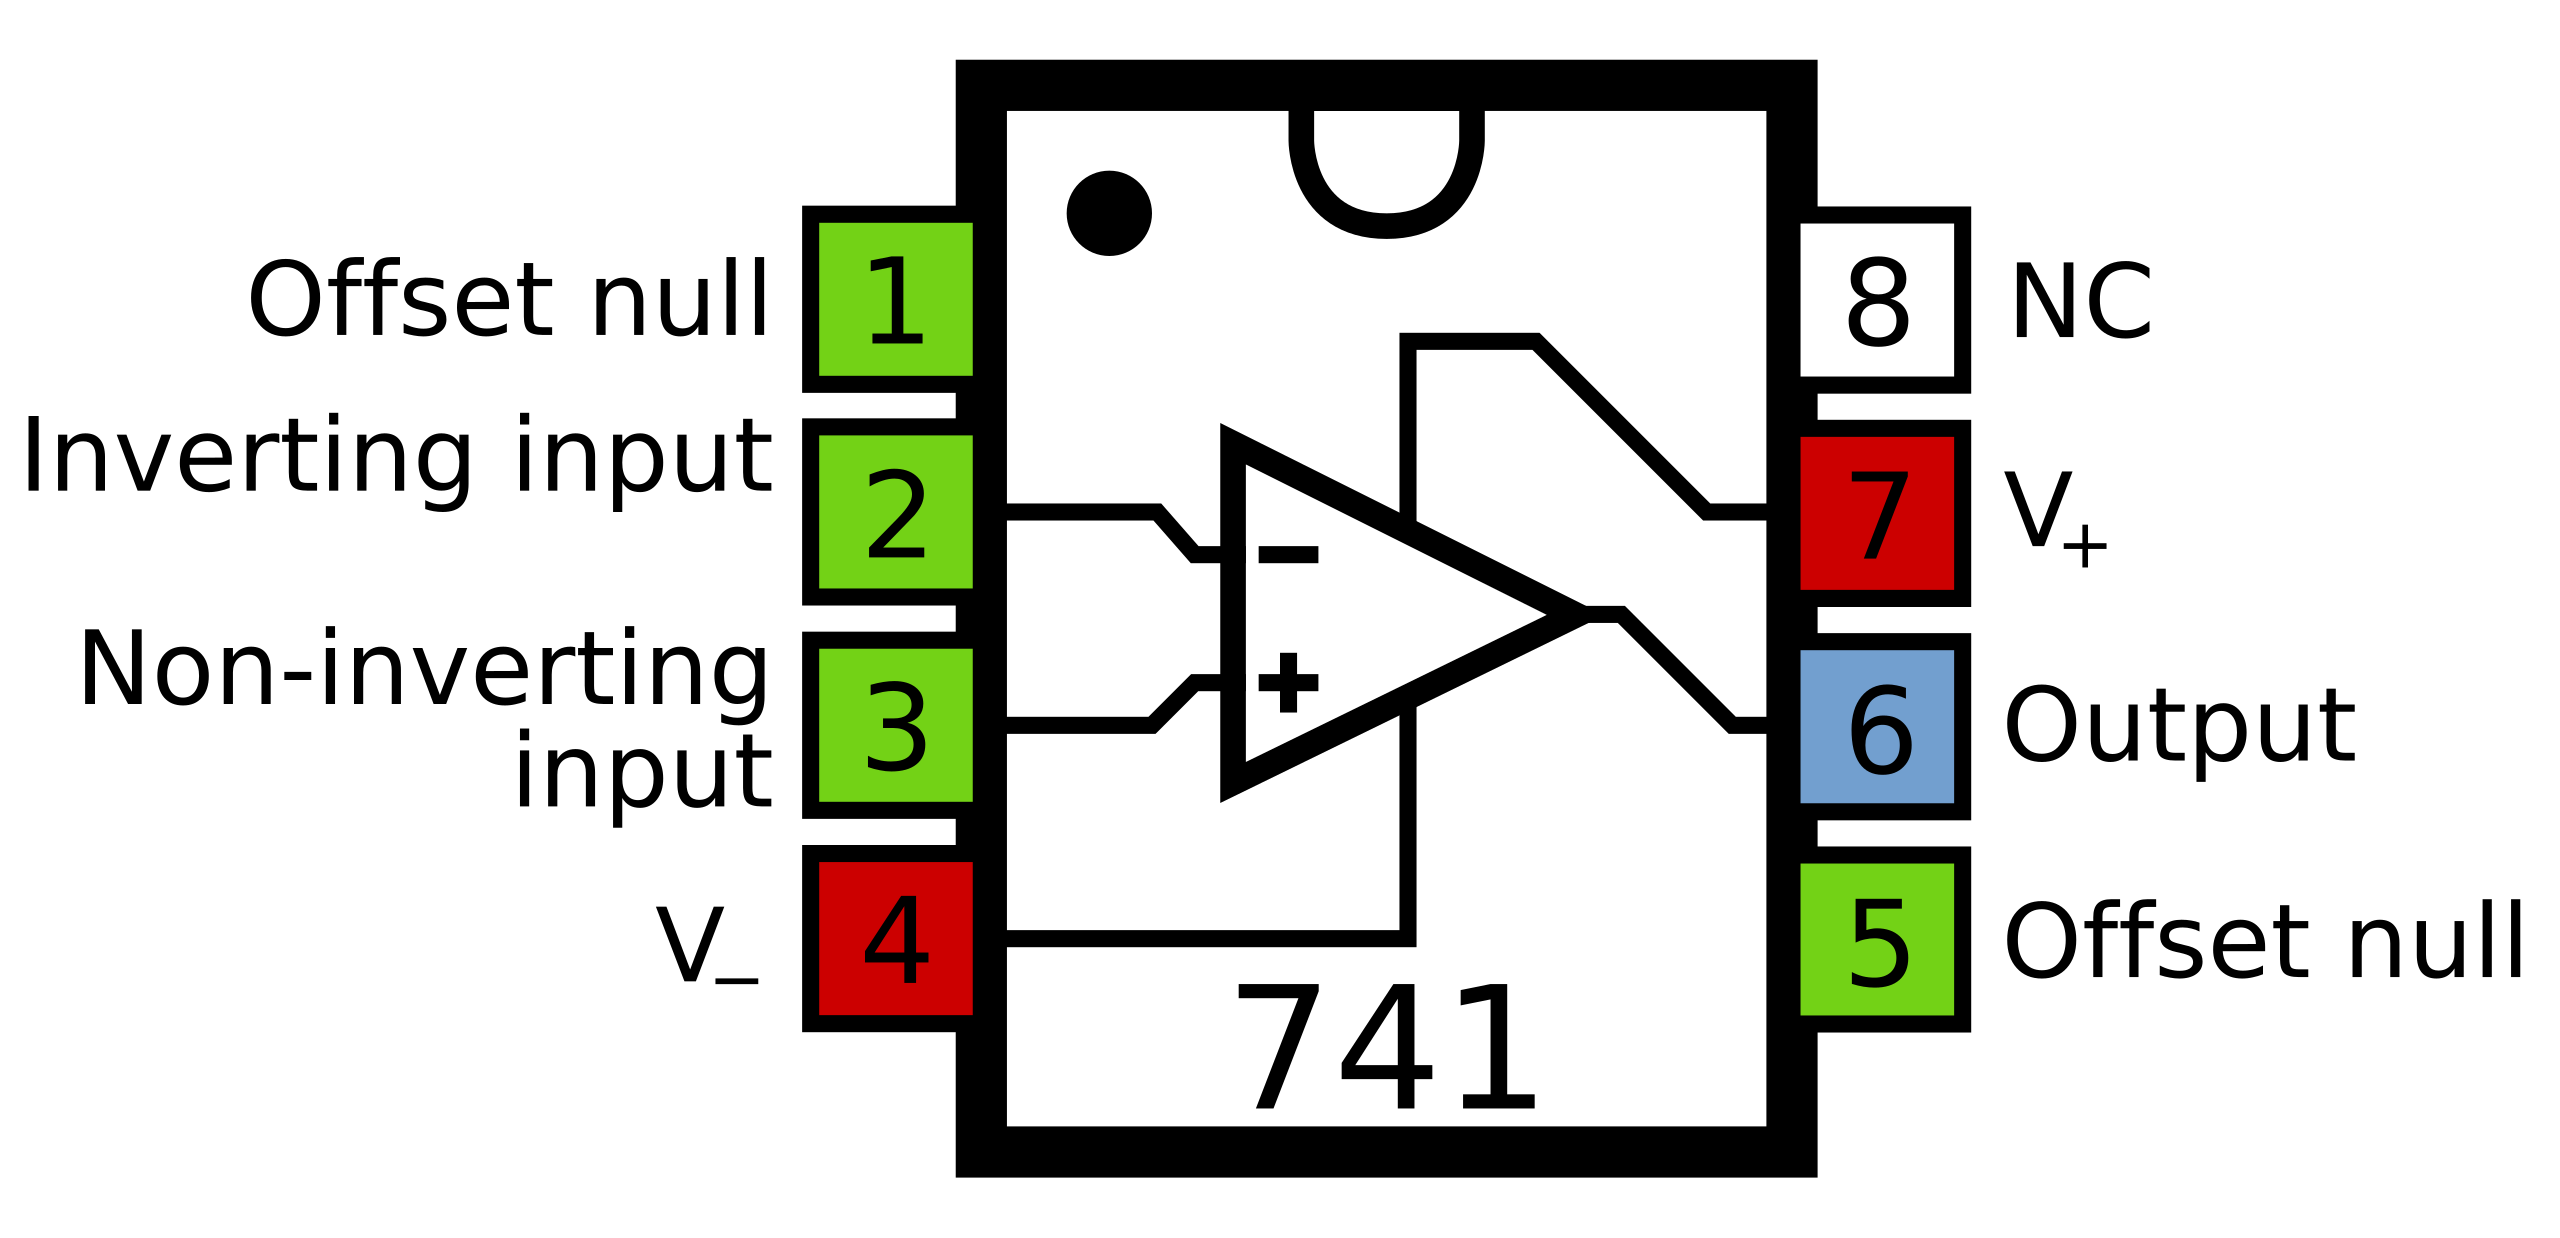
\includegraphics[width=0.5\textwidth]{LM741.png}
    \caption{LM741 pin configuration, Source :The Internet}
\end{figure}
The LM741 is a general-purpose operational amplifier.
Pins 2 and 3 are the inverting and non-inverting inputs respectively. Pin 4 is the negative power supply, pin 7 is the positive power supply and pin 6 is the output pin.
Pins 1 and 5 are the offset null pins. The offset null pins are used to nullify the offset voltage of the op-amp. The offset voltage is the voltage required to make the output voltage zero when the input voltage is zero.
Pin 8 is a no-connector pin. It is used to make the IC symmetric  and easier to fit on a breadboard and is not connected to anything.
In our experiment, we have used the LM741 opamp. The pin configuration of the LM741 is shown above.
\subsection{Inverting Amplifier}
The Inverting Amplifier takes in a input voltage and gives us an output voltage with the opposite sign and amplified as per 
the resistors connected in the circuit.
\begin{figure}[H]
    \centering
    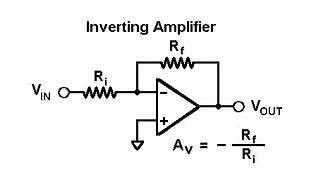
\includegraphics[width=0.5\textwidth]{invamp.jpg}
    \caption{Inverting Amplifier, Source :The Internet}
\end{figure}
The amplification or gain of the op-amp running in the inverting configuration is given by the
\begin{align*}
    A = -\frac{R_f}{R_i}
\end{align*}
where $R_f$ is the feedback resistor and $R_i$ is the input resistor.
\subsection{Non-Inverting Amplifier}
The non-inverting amplifier takes an input voltage and gives us an output voltage with the same sign and amplified as per the resistors connected in the circuit.
\begin{figure}[H]
    \centering
    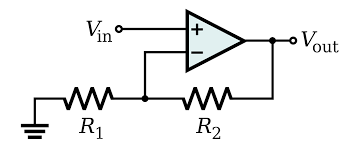
\includegraphics[width=0.5\textwidth]{noninv.png}
        \caption{Non-Inverting Amplifier, Source :The Internet}
\end{figure}

The amplification or gain of the op-amp running in the non-inverting configuration is given by the
\begin{align*}
    A = 1 + \frac{R_f}{R_i}
\end{align*}
where $R_f$ is the feedback resistor and $R_i$ is the input resistor.
\subsection{Adder}
The adder takes two or more voltages and adds them up in the output. The output voltage is the sum of the input voltages, provided all the resistors
connected in the circuit are equal. Otherwise, we get a weighted sum of the input voltages.

\begin{figure}[H]
    \centering
    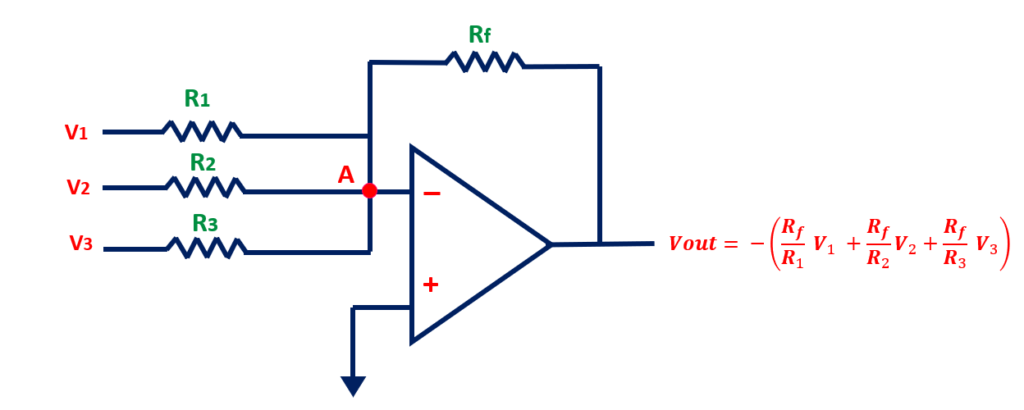
\includegraphics[width=0.5\textwidth]{adder.png}
    \caption{Adder, Source :The Internet}
\end{figure}

The output voltage of the adder is given by
\begin{align*}
    V_o = -\left(\frac{V_1}{R_1} + \frac{V_2}{R_2} + \frac{V_3}{R_3}\right)R_f
\end{align*}
where $V_1, V_2, V_3$ are the input voltages and $R_1, R_2, R_3$ are the resistors connected to the input voltages and $R_f$ is the feedback resistor.
\subsection{Subtractor}
The subtractor takes two input voltages and gives us the difference of the two voltages as the output. The output voltage is the difference of the two input voltages, provided all the resistors connected in the circuit are equal. Otherwise, we get a weighted difference of the input voltages.

\begin{figure}[H]
    \centering
    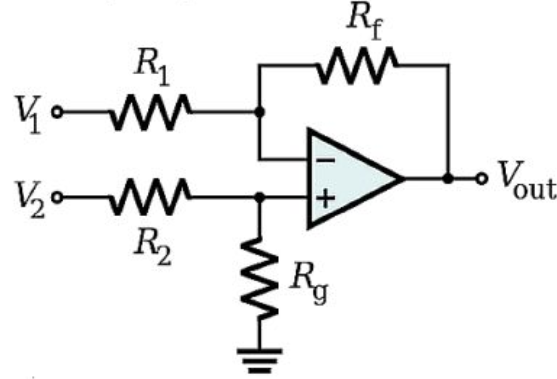
\includegraphics[width=0.5\textwidth]{sub.png}
    \caption{Subtractor, Source :The Internet}
\end{figure}

The output voltage of the subtractor is given by
\begin{align*}
    V_o = V_2 - V_1
\end{align*}
where $V_1, V_2$ are the input voltages and the resistors connected to the input voltages are equal, along with
the feedback resistor.

\section{Inverting Amplifier}
The data for the inverting amplifier is given in the supplementary section in \cref{inv}, Table 1. The data was collected by varying the input voltage and measuring the output voltage, over a range of 
$R_f/R_i$ ratios. The average gain for each configuration is
\begin{table}[H]
    \centering
    \caption{Average values and error}
    \begin{tabular}{|l|l|l|l|}
    \hline
        \textbf{-R\_f/R\_i} & \textbf{A(Theo.)} & \textbf{Average} & \textbf{Std. Dev} \\ \hline
        \textbf{-9.8/1} & -9.8 & -9.792 & 0.0016 \\ \hline
        \textbf{-9.8/2.16} & -4.537037037 & -4.549 & 0.00051 \\ \hline
        \textbf{-21.7/9.8} & -2.214285714 & -2.212 & 0.0005997 \\ \hline
        \textbf{-2.16/1} & -2.16 & -2.1625 & 0.000075 \\ \hline
        \textbf{-3.16/1} & -3.16 & -3.1750 & 0.00013 \\ \hline
    \end{tabular}
    \label{avg}
\end{table}
\section{Non-Inverting Amplifier}
The data for the non-inverting amplifier is given in the supplementary section in \cref{noninv}, Table 2. The data was collected by varying the input voltage and measuring the output voltage, over a range of
$R_f/R_i$ ratios. The average gain for each configuration is
\begin{table}[!ht]
    \centering
    \caption{Average values and error}
    \begin{tabular}{|l|l|l|l|}
    \hline
        \textbf{1 + R\_f/R\_i} & \textbf{A(Theo.)} & \textbf{Average} & \textbf{Std. Dev.} \\ \hline
        \textbf{1+2.16/1} & 3.16 & 3.155 & 0.0005 \\ \hline
        \textbf{1+9.08/1} & 10.08 & 10.895 & 0.0082 \\ \hline
        \textbf{1+21.7/9.8} & 3.214285714 & 3.2025 & 0.00048 \\ \hline
        \textbf{1+9.8/2.16} & 5.537037037 & 5.526 & 0.00098 \\ \hline
        \textbf{1+3.16} & 4.16 & 4.207 & 0.0037 \\ \hline
    \end{tabular}
    \label{avgnoninv}
\end{table}
\section{Adder}
The data for the adder is given in the supplementary section in \cref{adder}, Table 3. The data was collected by varying the input voltage and measuring the output voltage.
We then fit the data to a linear model to get the slope of the line which is the gain of the adder. The slope in theory should be one.
The plot of the linear fit is given here
\begin{figure}[H]
    \centering
    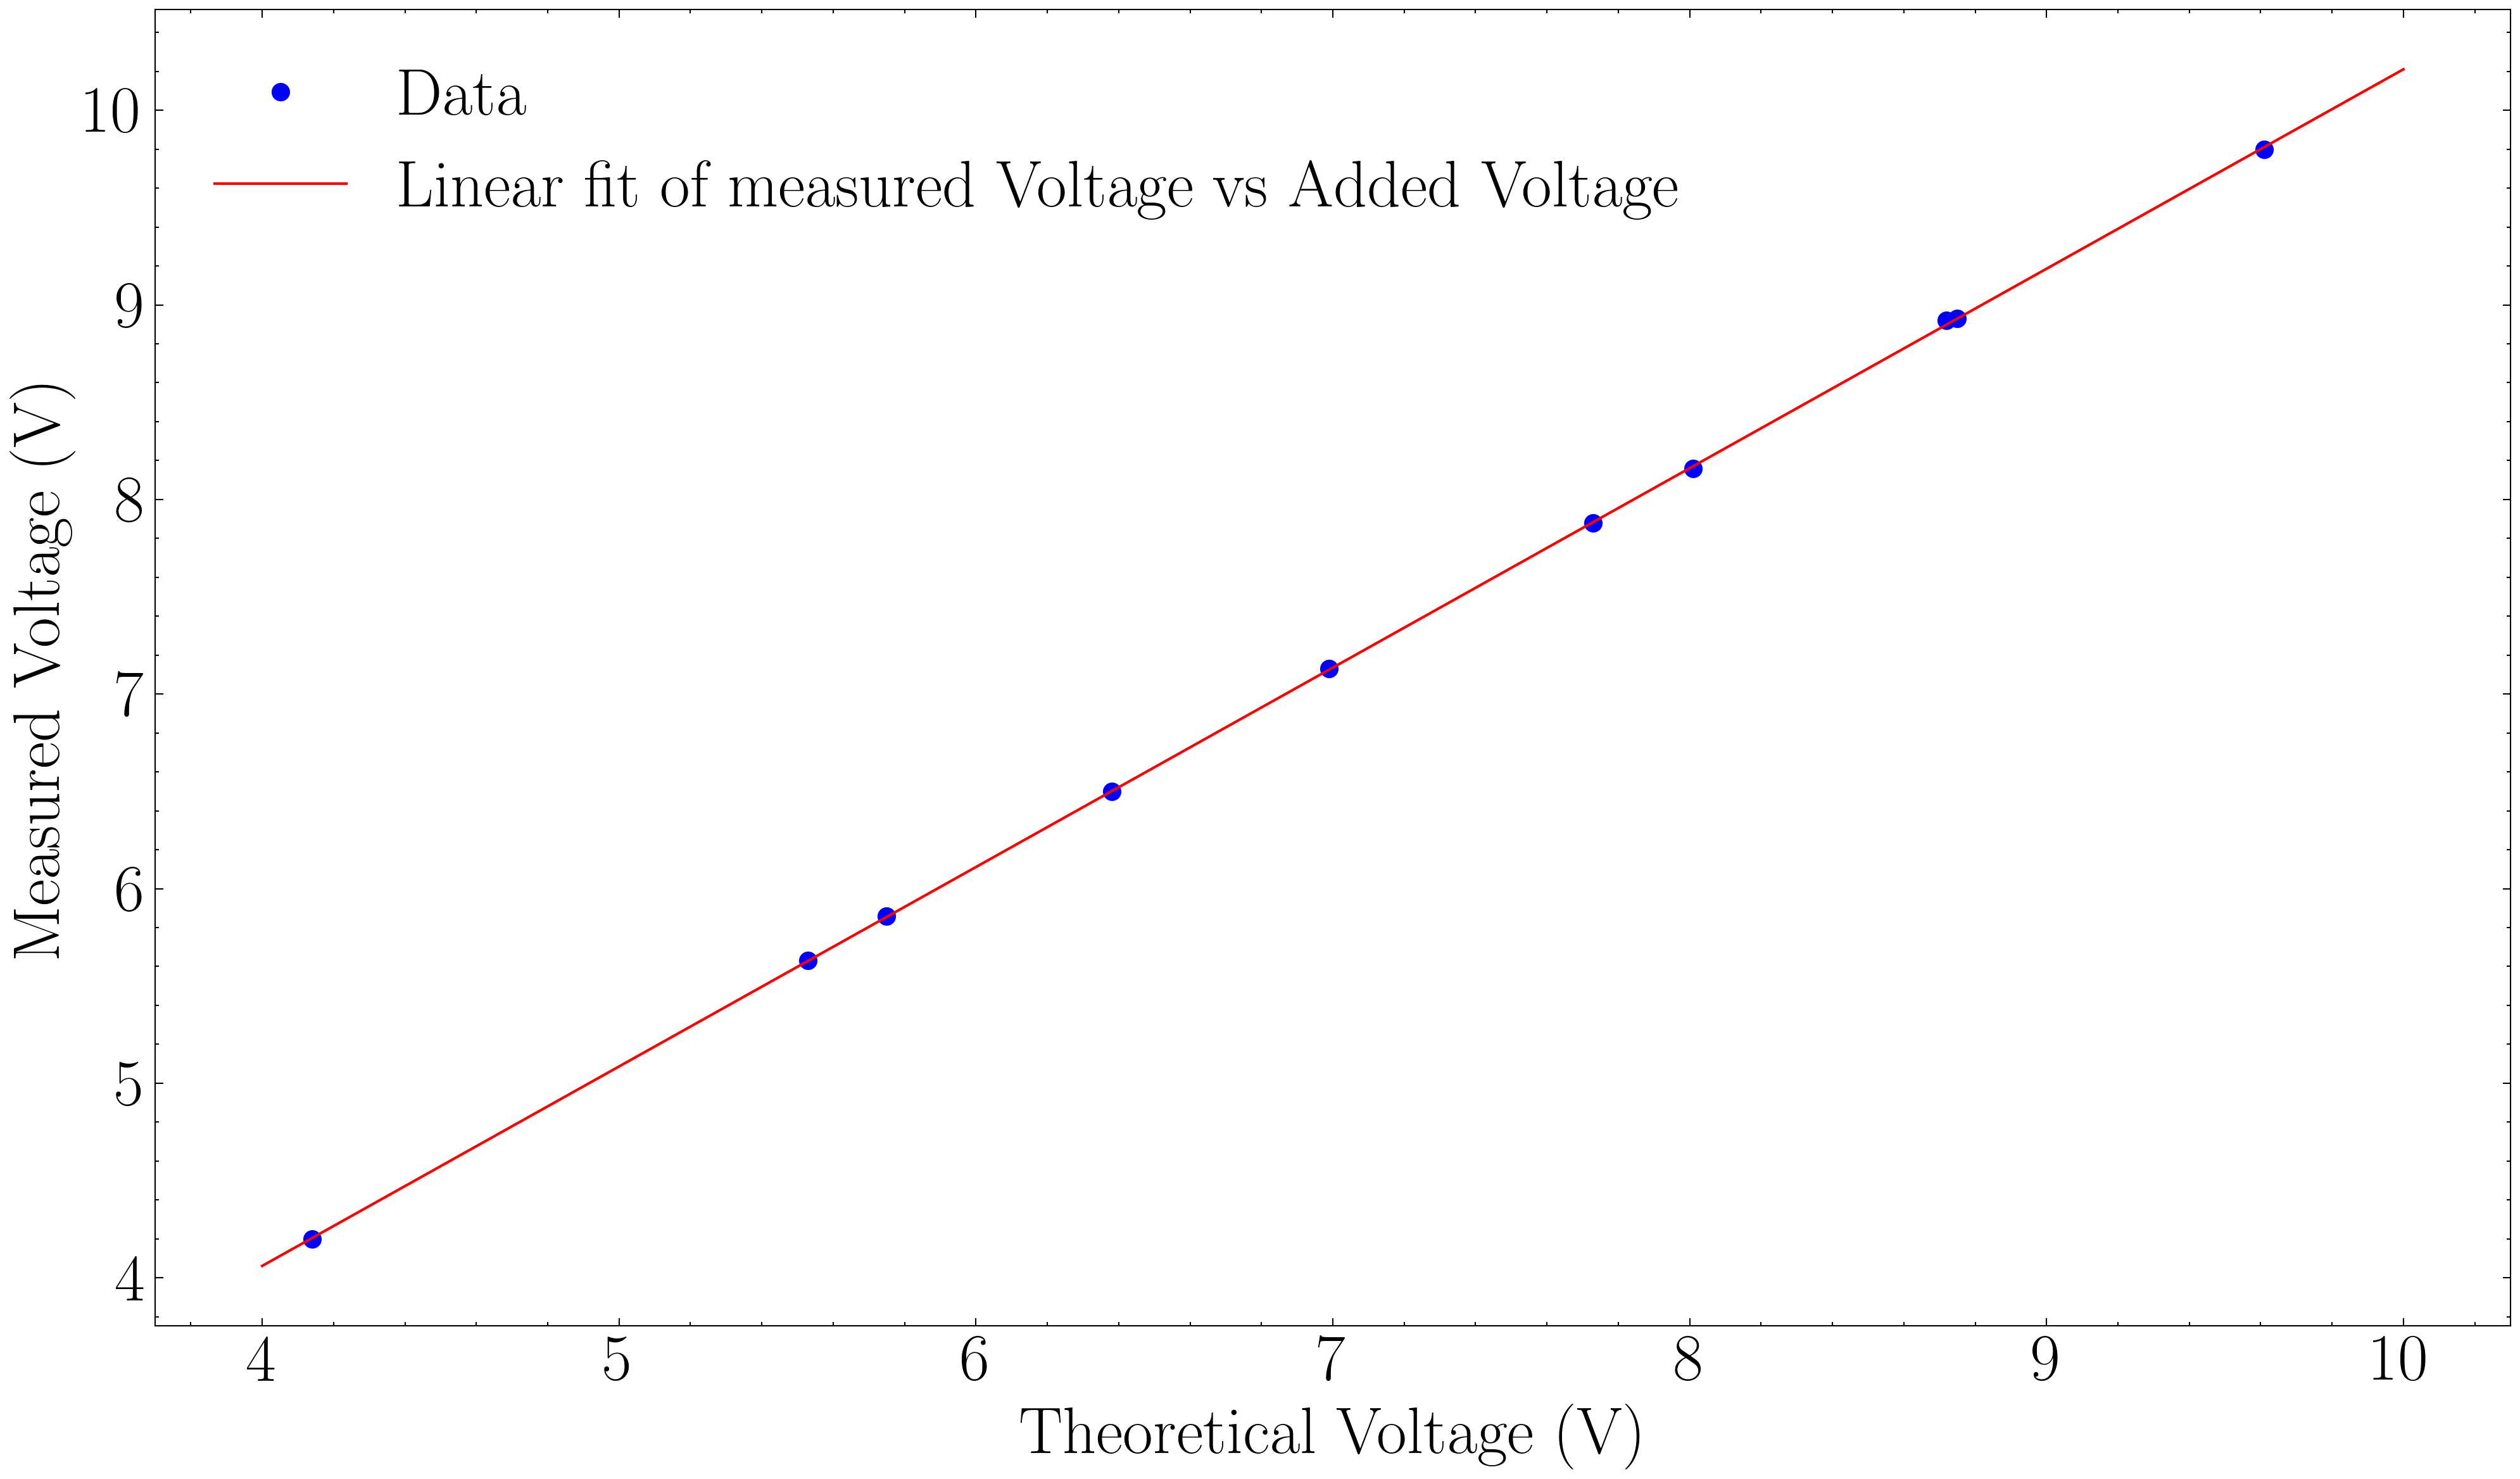
\includegraphics[width=0.8\textwidth]{Adder_plot.png}
    \caption{Adder linear fit}
\end{figure}
We expect the slope to be 1, but we get the slope as $\mathbf{1.02 \pm 0.0019}$. The error in slope could be due to errors in the measurement of 
the resistors connected to the circuit.
\section{Subtractor}
The data for the subtractor is given in the supplementary section in \cref{Sub}, Table 4. The data was collected by varying the input voltage and measuring the output voltage.
We then fit the data to a linear model to get the slope of the line which is the gain of the subtractor. The slope in theory should be one.
The plot of the linear fit is given here
\begin{figure}[H]
    \centering
    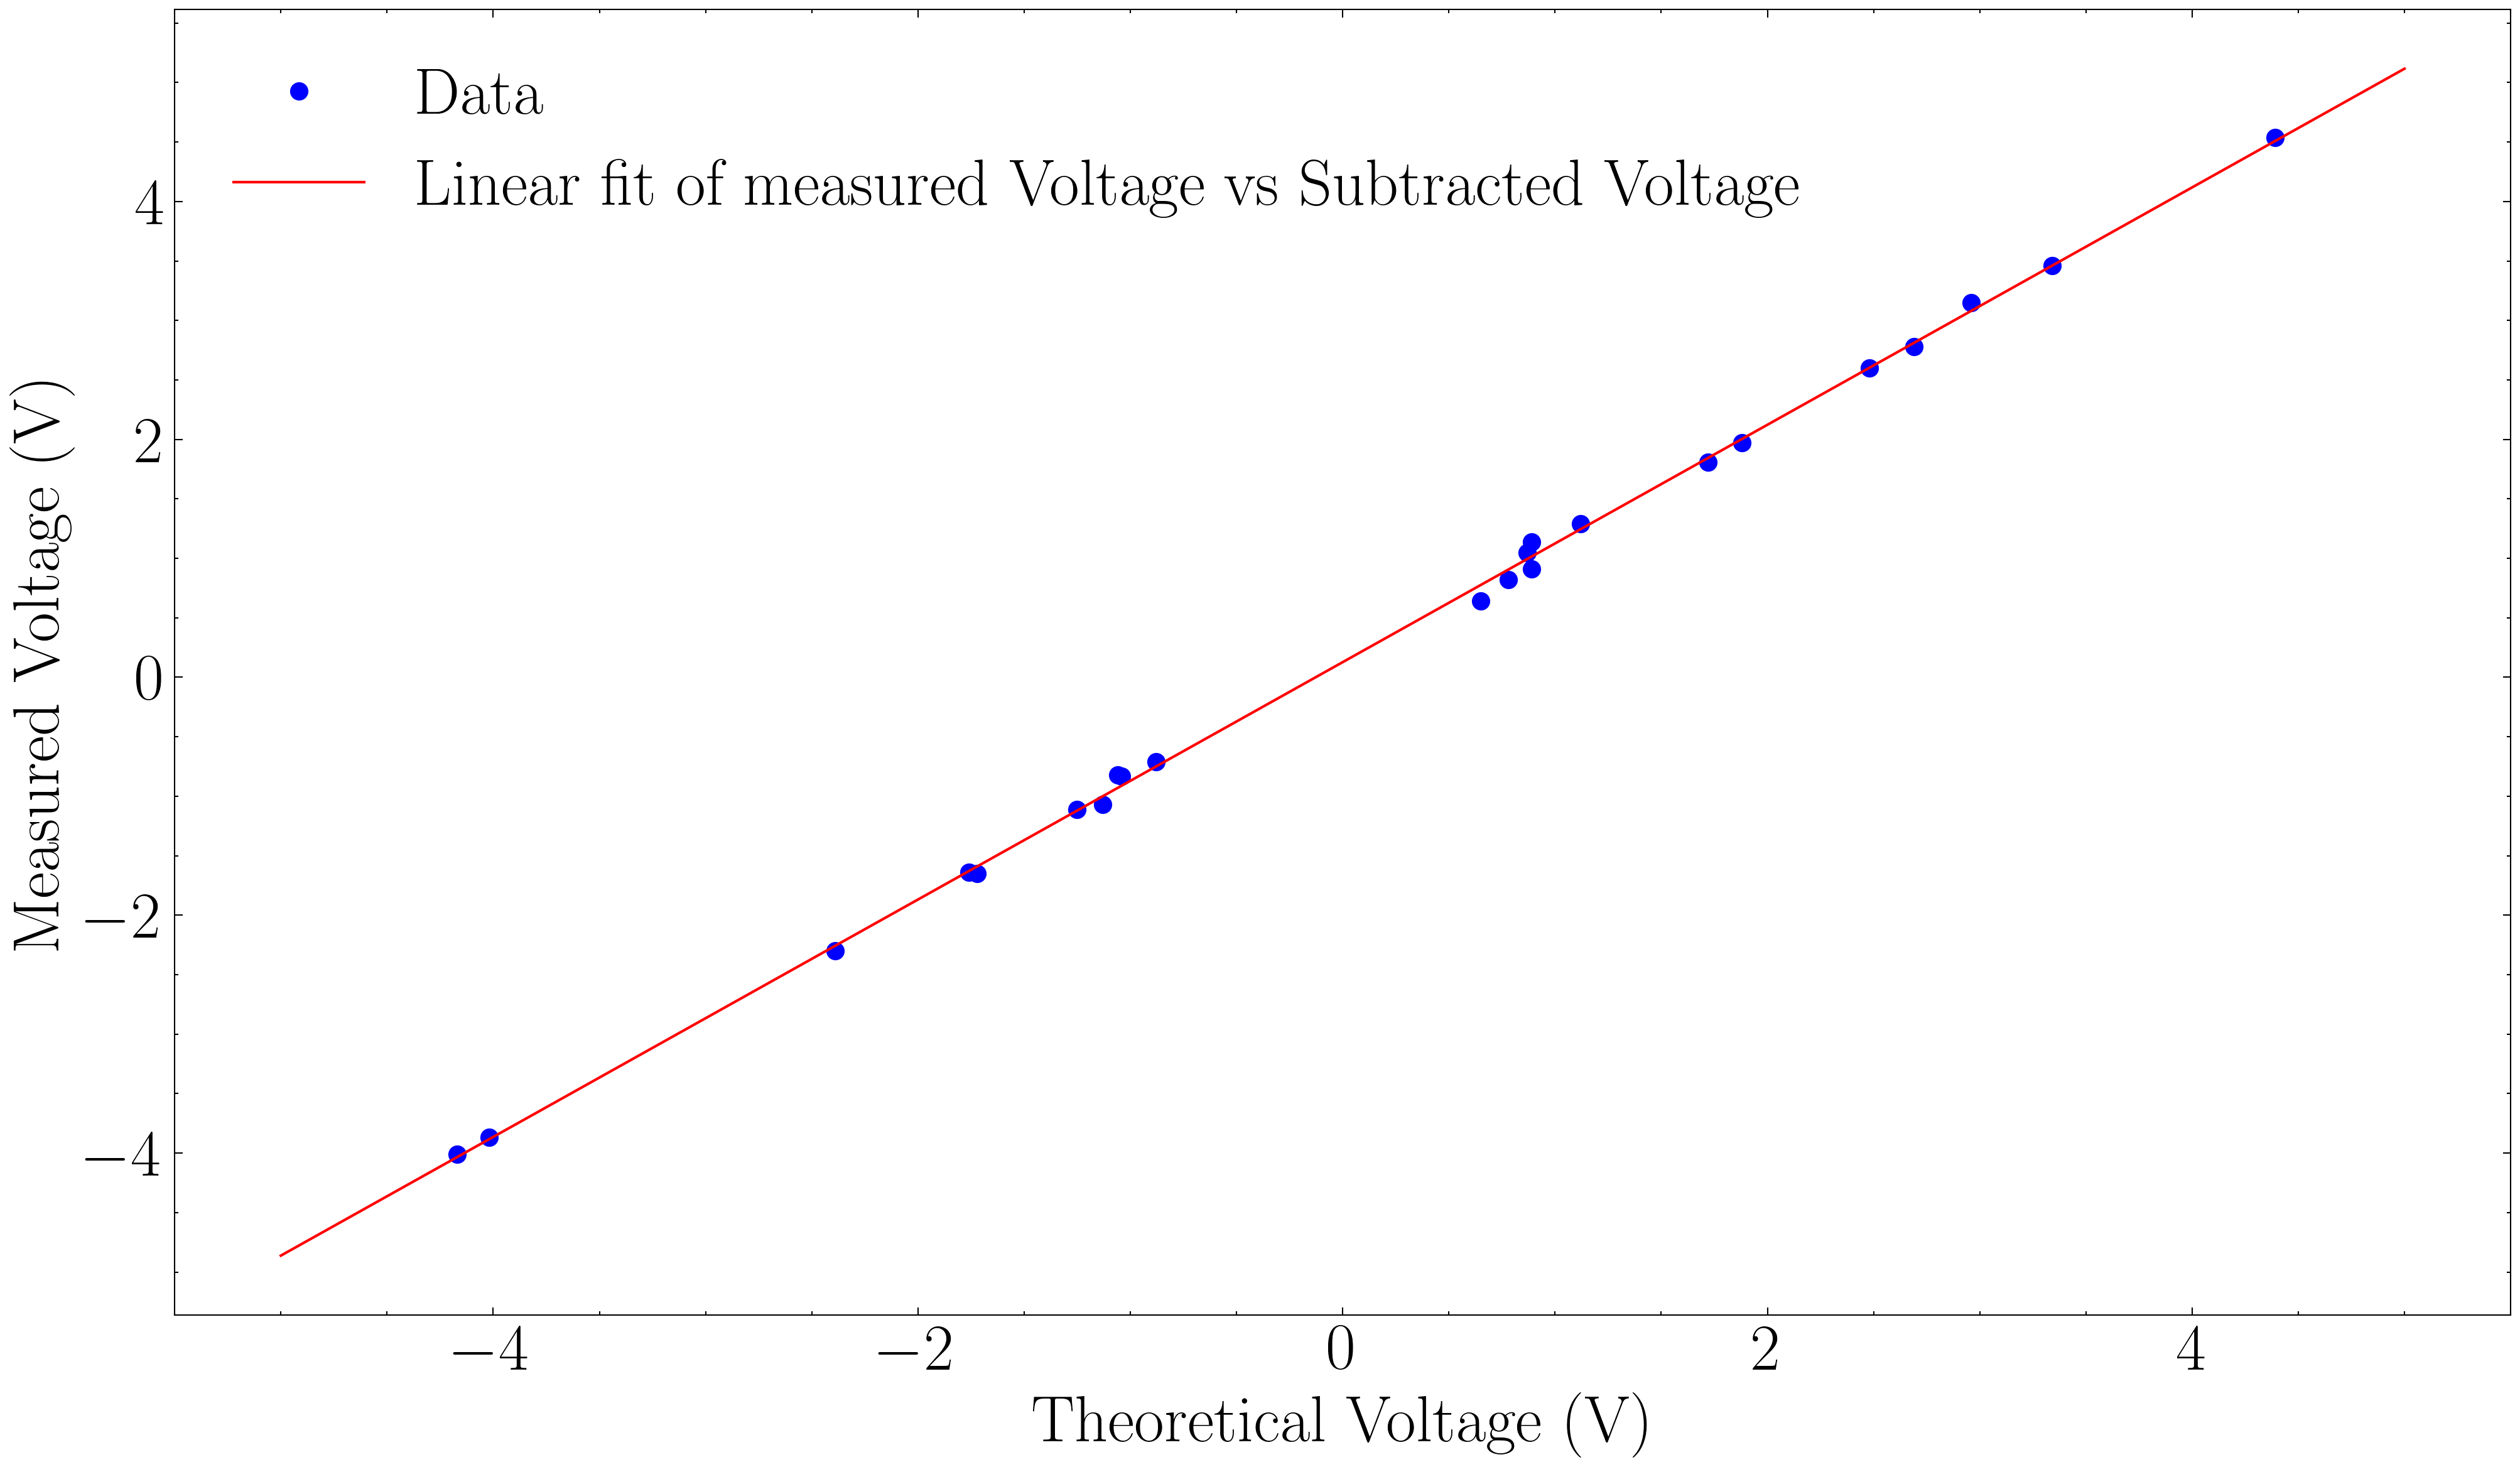
\includegraphics[width=0.8\textwidth]{Sub_plot.png}
    \caption{Subtractor linear fit}
\end{figure}
We get the slope to be $\mathbf{0.997 \pm 0.006} $ instead of $1$. The error in slope could be due to errors in the measurement of the resistors connected to the circuit.
\section{Results}
We can see that the theory in all the experiments matches up quite well with the experiments done in the lab. 
In the non inverting amplifier and the inverting amplifier, we see that the average gain is very close to the theoretical gain, in all the domains of the experiment,
both negative and positive values of input voltage. We can also see that in the case of the adder and the subtractor the experimental values are very close to the theoretical values.
\section{Error Analysis}
\begin{itemize}
    \item The least count of the multimeters are a source of error in the measurement of the input and output voltages and the resistors.
    \item The power supply could have a small error in the voltage supplied to the circuit.
    \item The op-amp might have had a small offset voltage which could have caused a small error in the output voltage.
\end{itemize}
\section{Conclusion}
    We conclude that the experiments done in the lab match up quite well with the theoretical values. The op-amp is a very useful component in electronics and has a wide range of applications.
\newpage
\section{Supplementary}
\begin{table}[!ht]
    \centering
    \begin{tabular}{|l|l|l|l|l|}
    \hline
        \textbf{-R\_f/R\_i} & \textbf{A(Theo.)} & \textbf{Vi(V)} & \textbf{Vo(V)} & \textbf{A(Expt)} \\ \hline
        \textbf{-9.8/1} & -9.8 & -0.5 & 4.9 & -9.8 \\ \hline
        \textbf{-9.8/1} & -9.8 & -0.99 & 9.67 & -9.767676768 \\ \hline
        \textbf{-9.8/1} & -9.8 & 0.5 & -4.91 & -9.82 \\ \hline
        \textbf{-9.8/1} & -9.8 & 1 & -9.78 & -9.78 \\ \hline
        \textbf{-9.8/2.16} & -4.537037037 & 1 & -4.56 & -4.56 \\ \hline
        \textbf{-9.8/2.16} & -4.537037037 & 0.5 & -2.28 & -4.56 \\ \hline
        \textbf{-9.8/2.16} & -4.537037037 & -0.99 & 4.49 & -4.535353535 \\ \hline
        \textbf{-9.8/2.16} & -4.537037037 & -0.5 & 2.27 & -4.54 \\ \hline
        \textbf{-21.7/9.8} & -2.214285714 & -0.49 & 1.09 & -2.224489796 \\ \hline
        \textbf{-21.7/9.8} & -2.214285714 & -1 & 2.2 & -2.2 \\ \hline
        \textbf{-21.7/9.8} & -2.214285714 & 0.49 & -1.09 & -2.224489796 \\ \hline
        \textbf{-21.7/9.8} & -2.214285714 & 1 & -2.2 & -2.2 \\ \hline
        \textbf{-2.16/1} & -2.16 & 1 & -2.16 & -2.16 \\ \hline
        \textbf{-2.16/1} & -2.16 & 0.5 & -1.08 & -2.16 \\ \hline
        \textbf{-2.16/1} & -2.16 & -1 & 2.17 & -2.17 \\ \hline
        \textbf{-2.16/1} & -2.16 & -0.5 & 1.08 & -2.16 \\ \hline
        \textbf{-3.16/1} & -3.16 & -1 & 3.17 & -3.17 \\ \hline
        \textbf{-3.16/1} & -3.16 & 0.51 & -1.62 & -3.176470588 \\ \hline
        \textbf{-3.16/1} & -3.16 & 1 & -3.17 & -3.17 \\ \hline
        \textbf{-3.16/1} & -3.16 & -0.49 & 1.56 & -3.183673469 \\ \hline
    \end{tabular}
    \label{inv}
    \caption{Inverting Amplifier}
\end{table}
\begin{table}[!ht]
    \centering
    \caption{Non Inverting Amplifier}
    \begin{tabular}{|l|l|l|l|l|}
    \hline
        \textbf{1 + R\_f/R\_i} & \textbf{A(Theo.)} & \textbf{Vi(V)} & \textbf{Vo(V)} & \textbf{A(Expt)} \\ \hline
        \textbf{1+2.16/1} & 3.16 & 1 & 3.17 & 3.17 \\ \hline
        \textbf{1+2.16/1} & 3.16 & 0.5 & 1.58 & 3.16 \\ \hline
        \textbf{1+2.16/1} & 3.16 & -1 & -3.15 & 3.15 \\ \hline
        \textbf{1+2.16/1} & 3.16 & -0.5 & -1.57 & 3.14 \\ \hline
        \textbf{1+9.08/1} & 10.08 & -0.49 & -5.36 & 10.93877551 \\ \hline
        \textbf{1+9.08/1} & 10.08 & -1 & -10.82 & 10.82 \\ \hline
        \textbf{1+9.08/1} & 10.08 & 0.5 & 5.46 & 10.92 \\ \hline
        \textbf{1+9.08/1} & 10.08 & 1 & 10.9 & 10.9 \\ \hline
        \textbf{1+21.7/9.8} & 3.214285714 & 1 & 3.2 & 3.2 \\ \hline
        \textbf{1+21.7/9.8} & 3.214285714 & 0.5 & 1.61 & 3.22 \\ \hline
        \textbf{1+21.7/9.8} & 3.214285714 & -1 & -3.19 & 3.19 \\ \hline
        \textbf{1+21.7/9.8} & 3.214285714 & -0.5 & -1.6 & 3.2 \\ \hline
        \textbf{1+9.8/2.16} & 5.537037037 & -0.5 & -2.75 & 5.5 \\ \hline
        \textbf{1+9.8/2.16} & 5.537037037 & -0.99 & -5.48 & 5.535353535 \\ \hline
        \textbf{1+9.8/2.16} & 5.537037037 & 0.5 & 2.77 & 5.54 \\ \hline
        \textbf{1+9.8/2.16} & 5.537037037 & 1 & 5.53 & 5.53 \\ \hline
        \textbf{1+3.16} & 4.16 & 0.99 & 4.2 & 4.242424242 \\ \hline
        \textbf{1+3.16} & 4.16 & 0.5 & 2.11 & 4.22 \\ \hline
        \textbf{1+3.16} & 4.16 & -0.99 & -4.16 & 4.202020202 \\ \hline
        \textbf{1+3.16} & 4.16 & -0.49 & -2.04 & 4.163265306 \\ \hline
    \end{tabular}
    \label{noninv}
\end{table}
\begin{table}[!ht]
    \centering
    \caption{Adder}
    \begin{tabular}{|l|l|l|l|l|l|l|}
    \hline
        \textbf{SL no.} & \textbf{V1(V)} & \textbf{V2(V)} & \textbf{V3(V)} & \textbf{} & \textbf{Vo(meas)} & \textbf{Vo(Theo)} \\ \hline
        \textbf{1} & 4.93 & 2.01 & 1.07 & 8.16 & -8.16 & 8.01 \\ \hline
        \textbf{2} & 5.91 & 2.42 & 1.28 & 9.8 & -9.8 & 9.61 \\ \hline
        \textbf{3} & 2.4 & 1.18 & 0.56 & 4.2 & -4.2 & 4.14 \\ \hline
        \textbf{4} & 3.94 & 1.58 & 0.86 & 6.5 & -6.5 & 6.38 \\ \hline
        \textbf{5} & 4 & 1.83 & 1.16 & 7.13 & -7.13 & 6.99 \\ \hline
        \textbf{6} & 3.28 & 1.45 & 0.8 & 5.63 & -5.63 & 5.53 \\ \hline
        \textbf{7} & 3.34 & 1.64 & 0.77 & 5.86 & -5.86 & 5.75 \\ \hline
        \textbf{8} & 5.12 & 2.57 & 1.06 & 8.93 & -8.93 & 8.75 \\ \hline
        \textbf{9} & 4.49 & 2.2 & 1.04 & 7.88 & -7.88 & 7.73 \\ \hline
        \textbf{10} & 5.7 & 2.13 & 0.89 & 8.92 & -8.92 & 8.72 \\ \hline
    \end{tabular}
    \label{adder}
\end{table}
\begin{table}[!ht]
    \centering
    \caption{Subtractor}
    \begin{tabular}{|l|l|l|l|l|}
    \hline
        \textbf{SL. no.} & \textbf{V1(V)} & \textbf{V2(V)} & \textbf{Vo(Meas)} & \textbf{Vo(Theo)} \\ \hline
        \textbf{1} & 0.15 & 1.04 & 0.91 & 0.89 \\ \hline
        \textbf{2} & 0.26 & 1.04 & 0.82 & 0.78 \\ \hline
        \textbf{3} & 0.39 & 1.04 & 0.64 & 0.65 \\ \hline
        \textbf{4} & 1.12 & 3 & 1.97 & 1.88 \\ \hline
        \textbf{5} & 1.39 & 3.11 & 1.81 & 1.72 \\ \hline
        \textbf{6} & 1.59 & 4.07 & 2.6 & 2.48 \\ \hline
        \textbf{7} & 0.86 & 3.55 & 2.78 & 2.69 \\ \hline
        \textbf{8} & 3.02 & 5.98 & 3.15 & 2.96 \\ \hline
        \textbf{9} & 1.41 & 5.8 & 4.54 & 4.39 \\ \hline
        \textbf{10} & 1.08 & 4.42 & 3.46 & 3.34 \\ \hline
        \textbf{11} & 5.31 & 6.2 & 1.14 & 0.89 \\ \hline
        \textbf{12} & 3.69 & 4.56 & 1.05 & 0.87 \\ \hline
        \textbf{13} & 3.34 & 4.46 & 1.29 & 1.12 \\ \hline
        \textbf{14} & 4.13 & 3.25 & -0.71 & -0.88 \\ \hline
        \textbf{15} & 4.85 & 3.81 & -0.83 & -1.04 \\ \hline
        \textbf{16} & 5.79 & 4.73 & -0.82 & -1.06 \\ \hline
        \textbf{17} & 3.36 & 1.6 & -1.64 & -1.76 \\ \hline
        \textbf{18} & 3.5 & 2.25 & -1.11 & -1.25 \\ \hline
        \textbf{19} & 5.32 & 1.15 & -4.01 & -4.17 \\ \hline
        \textbf{20} & 5.13 & 1.11 & -3.87 & -4.02 \\ \hline
        \textbf{21} & 3.05 & 0.66 & -2.3 & -2.39 \\ \hline
        \textbf{22} & 2.19 & 0.47 & -1.65 & -1.72 \\ \hline
        \textbf{23} & 1.43 & 0.3 & -1.07 & -1.13 \\ \hline
    \end{tabular}
    \label{Sub}
\end{table}

\end{document}
